\documentclass{article}
\usepackage{amsmath, sfmath, multicol, tkz-euclide, array, enumerate, tcolorbox, tabularray}
\renewcommand{\familydefault}{\sfdefault}
\setlength{\parindent}{0cm}
\pagestyle{empty}
\usepackage[left=1in, top=0.5in, right=1in, bottom=0.5in]{geometry}
\tikzset{>=stealth}
\tcbset{colback=white}

\newcounter{example}[section]
\newenvironment{example}[1][]{\refstepcounter{example}\par\medskip
   {\color{red}\textbf{Example~\theexample. #1}}}{\medskip}

\begin{document}

\section*{Proportions in Triangles}

\begin{tcolorbox}[colframe=orange!70!white, coltitle=black, title=\textbf{Today I Can}]
\begin{enumerate}
    \item Use the side-splitter theorem.
    \item Use the triangle angle-bisector theorem.
\end{enumerate}
\end{tcolorbox}
\smallskip

\begin{tcolorbox}[colframe=black!20!white, opacitybacktitle=0.1, coltitle=black, title=\textbf{Side-Splitter Theorem}]
If a segment is drawn inside a triangle parallel to the other side, then it divides the segments it intersects proportionally. \newline 

\begin{minipage}{0.4\textwidth}
\begin{itemize}
    \item If $\overline{RS} \parallel \overline{XY}$ then $\frac{XR}{RQ} = \frac{YS}{SQ}$. 
\end{itemize}
\end{minipage}
\begin{minipage}{0.5\textwidth}
    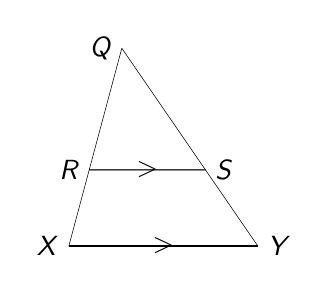
\begin{tikzpicture}[scale=0.8]
    \tkzDefPoints{0/0/X, 3/0/Y}
    \tkzDefShiftPoint[X](75:3.25){Q}
    \tkzDrawPolygon(X,Q,Y)
    \tkzDefShiftPoint[X](75:1.25){R}
    \tkzDefLine[parallel=through R](X,Y)
    \tkzGetPoint{T}
    \tkzInterLL(R,T)(Q,Y)
    \tkzGetPoint{S}
    \tkzDrawSegment(R,S)
    \tkzLabelPoints[left](Q,R,X)
    \tkzLabelPoints[right](S,Y)
    \draw (R) -- (S) node [midway] {$>$};
    \draw (X) -- (Y) node [midway] {$>$};
    \end{tikzpicture}
\end{minipage}
\end{tcolorbox}
\smallskip 

\begin{example}
Find the value of the variable in each.
\begin{multicols}{2}
\begin{enumerate}[(a)]
    \item \mbox{} \newline 
    \item \mbox{} \newline 
\end{enumerate}
\end{multicols}
\begin{minipage}{0.5\textwidth}
    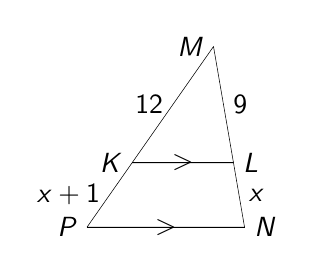
\begin{tikzpicture}[scale=0.8]
    \tkzDefPoints{0/0/P, 2.5/0/N}
    \tkzDefShiftPoint[P](55:3.5){M}
    \tkzDefShiftPoint[P](55:1.25){K}
    \tkzDrawPolygon(P,N,M)
    \tkzDefLine[parallel = through K](P,N)
    \tkzGetPoint{O}
    \tkzInterLL(K,O)(M,N)
    \tkzGetPoint{L}
    \tkzDrawSegment(K,L)
    \tkzLabelPoints[left](P,K,M)
    \tkzLabelPoints[right](L,N)
    \tkzLabelSegment[left](P,K){$x+1$}
    \tkzLabelSegment[left](K,M){12}
    \tkzLabelSegment[right](L,N){$x$}
    \tkzLabelSegment[right](L,M){9}
    \draw (P) -- (N) node [midway] {$>$};
    \draw (K) -- (L) node [midway] {$>$};
    \end{tikzpicture}
\end{minipage}
\begin{minipage}{0.4\textwidth}
    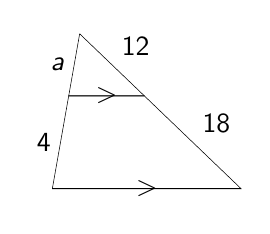
\begin{tikzpicture}[scale=0.8]
    \tkzDefPoints{0/0/A, 3/0/B}
    \tkzDefShiftPoint[A](80:2.5){C}
    \tkzDefShiftPoint[A](80:1.5){D}
    \tkzDefLine[parallel = through D](A,B)
    \tkzGetPoint{E}
    \tkzInterLL(D,E)(B,C)
    \tkzGetPoint{F}
    \tkzDrawSegment(D,F)
    \draw (A) -- (B) node [midway] {$>$};
    \draw (D) -- (F) node [midway] {$>$};
    \tkzLabelSegment[left](D,C){$a$}
    \tkzLabelSegment[left](A,D){4}
    \tkzLabelSegment[above right](F,C){12}
    \tkzLabelSegment[above right](B,F){18}
    \tkzDrawPolygon(A,B,C)
    \end{tikzpicture}
\end{minipage}
\end{example}

\vfill 

\begin{tcolorbox}[colframe=black!20!white, opacitybacktitle=0.1, coltitle=black, title=\textbf{Corollary to Side-Splitter Theorem}]

\begin{minipage}{0.5\textwidth}
\begin{itemize}
    \item If $a \parallel b \parallel c$
    \item Then $\frac{AB}{BC}=\frac{AE}{EF};  \quad   \frac{BC}{CD}=\frac{EF}{FG};   \quad   \frac{AB}{CD}=\frac{AE}{FG}$
\end{itemize}
\end{minipage}
\begin{minipage}{0.5\textwidth}
    \begin{tikzpicture}[scale=0.7]
    \tkzDefPoints{0/0/D, 3/0/G}
    \tkzDefShiftPoint[D](70:4){A}
    \tkzDefShiftPoint[D](70:2.5){B}
    \tkzDefShiftPoint[D](70:1.25){C}
    \tkzDrawSegments[dashed, add=0.35 and 0](D,A G,A)
    \tkzDrawSegment[add = 0.5 and 0.5, dashed](D,G)
    \tkzDefLine[parallel=through B](D,G)
    \tkzGetPoint{Z}
    \tkzInterLL(B,Z)(G,A)   \tkzGetPoint{E}
    \tkzDrawSegment[add=1in and 1in, dashed](B,E)
    \tkzDefLine[parallel=through C](D,G)
    \tkzGetPoint{Y}
    \tkzInterLL(C,Y)(G,A)   \tkzGetPoint{F}
    \tkzDrawSegment[add=0.85in and 0.85in, dashed](C,F)
    \tkzLabelPoints[above](A)
    \tkzLabelPoints[below left](D,C,B)
    \tkzLabelPoints[below right](G,F,E)
    \tkzLabelSegment[left, xshift=-1in](B,E){$a$}
    \tkzLabelSegment[left, xshift=-1in](C,F){$b$}
    \tkzLabelSegment[left, xshift=-1in](D,G){$c$}
    \end{tikzpicture}
\end{minipage}
\end{tcolorbox}
\smallskip 

\newpage 

\begin{tcolorbox}[colframe=black!20!white, opacitybacktitle=0.1, coltitle=black, title=\textbf{Triangle Angle-Bisector Theorem}]
The angle bisector of a triangle divides the sides of the triangle proportionally. \newline 

\begin{minipage}{0.5\textwidth}
\begin{itemize}
    \item If $\overline{AD} \text{ bisects } \angle CAB$ then $\frac{BD}{BA} = \frac{CD}{CA}$
\end{itemize}
\end{minipage}
\begin{minipage}{0.5\textwidth}
    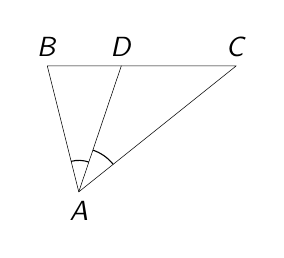
\begin{tikzpicture}[scale=0.8]
    \tkzDefPoints{0/0/B, 3/0/C, 0.5/-2/A}
    \tkzDrawPolygon(A,B,C)
    \tkzDefLine[bisector](B,A,C)    \tkzGetPoint{a}
    \tkzInterLL(A,a)(B,C)
    \tkzGetPoint{D}
    \tkzDrawSegment(A,D)
    \tkzMarkAngle[size=0.5](D,A,B)
    \tkzMarkAngle[size=0.7](C,A,D)
    \tkzLabelPoints[above](B,D,C)
    \tkzLabelPoints[below](A)
    \end{tikzpicture}
\end{minipage}
\end{tcolorbox}
\smallskip 

\begin{example}
What is the value of the variable in each? 

\begin{multicols}{2}
\begin{enumerate}[(a)]
    \item \mbox{} \newline 
    \item \mbox{} \newline 
\end{enumerate}
\end{multicols}
\begin{minipage}{0.5\textwidth}
    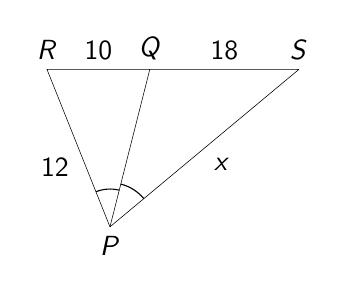
\begin{tikzpicture}[scale=0.8]
    \tkzDefPoints{0/0/R, 4/0/S, 1/-2.5/P}
    \tkzDrawPolygon(P,R,S)
    \tkzDefLine[bisector](R,P,S)    \tkzGetPoint{a}
    \tkzInterLL(P,a)(R,S)
    \tkzGetPoint{Q}
    \tkzDrawSegment(P,Q)
    \tkzMarkAngle[size=0.6](Q,P,R)
    \tkzMarkAngle[size=0.7](S,P,Q)
    \tkzLabelPoints[above](R,Q,S)
    \tkzLabelPoints[below](P)
    \tkzLabelSegment[below left](P,R){12}
    \tkzLabelSegment[above](R,Q){10}
    \tkzLabelSegment[above](S,Q){18}
    \tkzLabelSegment[below right](P,S){$x$}
    \end{tikzpicture}
\end{minipage}
\begin{minipage}{0.4\textwidth}
    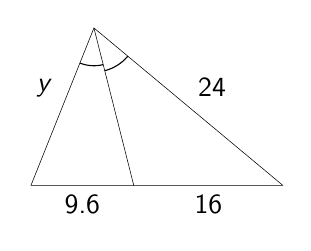
\begin{tikzpicture}[scale=0.8]
    \tkzDefPoints{0/0/R, 4/0/S, 1/2.5/P}
    \tkzDrawPolygon(P,R,S)
    \tkzDefLine[bisector](R,P,S)    \tkzGetPoint{a}
    \tkzInterLL(P,a)(R,S)
    \tkzGetPoint{Q}
    \tkzDrawSegment(P,Q)
    \tkzMarkAngle[size=0.6](R,P,Q)
    \tkzMarkAngle[size=0.7](Q,P,S)
    \tkzLabelSegment[above left](P,R){$y$}
    \tkzLabelSegment[below](R,Q){9.6}
    \tkzLabelSegment[below](S,Q){16}
    \tkzLabelSegment[above right](P,S){24}
    \end{tikzpicture}
\end{minipage}
\end{example}

\end{document}
